\documentclass{article}
\usepackage{tikz}
\usetikzlibrary{datavisualization}
\usetikzlibrary{datavisualization.formats.functions}
\usepackage{pgfplots}
\begin{document}
	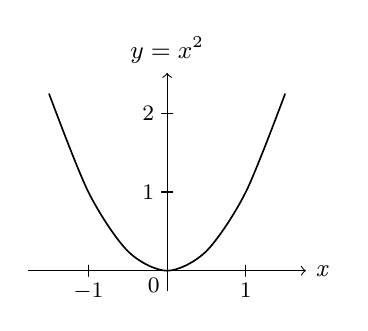
\begin{tikzpicture}
	\datavisualization [school book axes,
	visualize as smooth line,
	y axis={label={$y=x^2$}},
	x axis={label} ]
	
	data [format=function] {
		var x : interval [-1.5:1.5] samples 7;
		func y = \value x*\value x;
	};
	\end{tikzpicture}
	
	\vspace{2cm}
	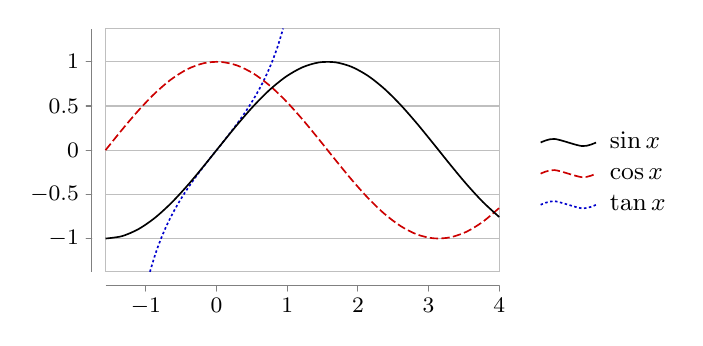
\begin{tikzpicture}
	\datavisualization [scientific axes=clean,
	y axis=grid,
	visualize as smooth line/.list={sin,cos,tan},
	style sheet=strong colors,
	style sheet=vary dashing,
	sin={label in legend={text=$\sin x$}},
	cos={label in legend={text=$\cos x$}},
	tan={label in legend={text=$\tan x$}},
	data/format=function
	]
	data [set=sin] {
		var x : interval [-0.5*pi:4];
		func y = sin(\value x r);
	}
	data [set=cos] {
		var x : interval [-0.5*pi:4];
		func y = cos(\value x r);
	}
	data [set=tan] {
		var x : interval [-0.3*pi:.3*pi];
		func y = tan(\value x r);
	};
	\end{tikzpicture}
	
	\vspace{2cm}
	\begin{tikzpicture}
		\begin{axis}[xmin=0,ymin=0,xmax=5,ymax=5,xtick distance=1.5,ytick distance=1.5,height=7cm,width=7cm,xlabel=rashi,ylabel=paul,title=mygraph,legend entries={$y=x$,$y=x/3$},legend style={font=\large,legend pos=outer north east,draw=none}]
		\addplot[domain=1.5:4.5,mark=+,samples=4,mark options={green},mark size=3pt] expression{x};
		\addplot expression{x/3};			
		\end{axis}
	\end{tikzpicture}\\
	\vspace{2cm}
	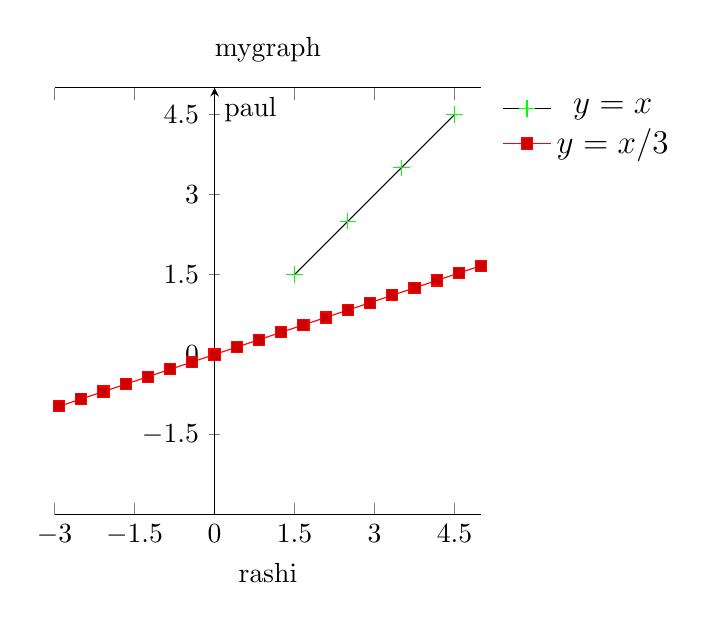
\begin{tikzpicture}
	\begin{axis}[axis y line=center,xmin=-3,ymin=-3,xmax=5,ymax=5,xtick distance=1.5,ytick distance=1.5,height=7cm,width=7cm,xlabel=rashi,ylabel=paul,title=mygraph,legend entries={$y=x$,$y=x/3$},legend style={font=\large,legend pos=outer north east,draw=none}]
	\addplot[domain=1.5:4.5,mark=+,samples=4,mark options={green},mark size=3pt] expression{x};
	\addplot expression{x/3};			
	\end{axis}
	\end{tikzpicture}\\
	\vspace{2cm}
	\begin{tikzpicture}
	\begin{axis}[axis x line=center,xmin=-3,ymin=-3,xmax=5,ymax=5,xtick distance=1.5,ytick distance=1.5,height=7cm,width=7cm,xlabel=rashi,ylabel=paul,title=mygraph,legend entries={$y=x$,$y=x/3$},legend style={font=\large,legend pos=outer north east,draw=none}]
	\addplot[domain=1.5:4.5,mark=+,samples=4,mark options={green},mark size=3pt] expression{x} node[midway,sloped,above] {hey yo};
	\addplot[mark=none,range=0:1] expression{x/3};			
	\end{axis}
	\end{tikzpicture}\\
	%Function by cases
	\vspace{2cm}
	\begin{tikzpicture}
	\begin{axis}[height=10cm,width=10cm]
	\addplot[smooth,samples=200,domain=-2:0]{0};
	\addplot[smooth,samples=200,domain=0:0.5]{x^2};
	\addplot[smooth,samples=200,domain=0.5:1]{1-3*(1-x)^2};
	\addplot[smooth,samples=200,domain=1:2]{1};
	\end{axis}
	\end{tikzpicture}\\
	\vspace{2cm}
	\begin{tikzpicture}
	\begin{axis}[axis lines=center,xmin=-3,ymin=-3,xmax=5,ymax=5,xtick distance=1.5,ytick distance=1.5,height=7cm,width=7cm,xlabel=rashi,ylabel=paul,title=mygraph,legend entries={$y=x^2+3*x+1$},legend style={font=\large,legend pos=outer north east,draw=none}]
	\addplot[mark=+,samples=50,mark options={green},mark size=3pt] {x^2 + 3*x + 1} ;
%	\addplot expression{x/3};	
	\addplot+ coordinates{(-2,2)(0,0)(2,2)};
		
	\end{axis}
	\end{tikzpicture}\\
	\vspace{2cm}
	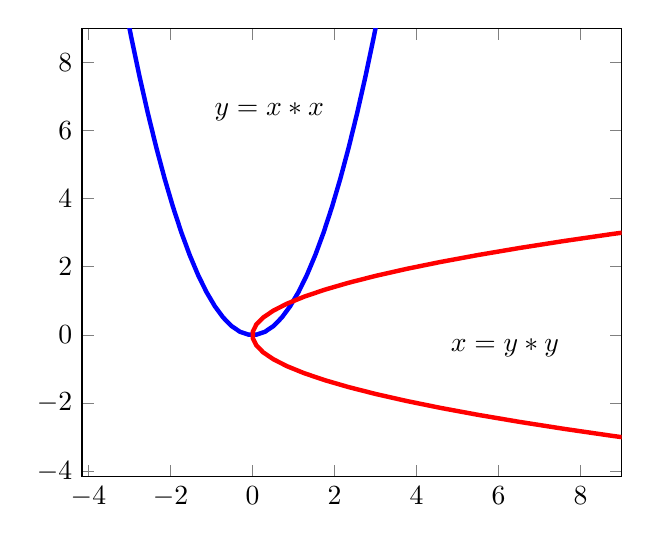
\begin{tikzpicture}
	\begin{axis}[xmax=9,ymax=9, samples=50]
	\addplot[blue, ultra thick] (x,x*x);
	\addplot[red,  ultra thick] (x*x,x);
	%\node[above=2cm,right=2cm]($y=x*x$);
	\node[above=5cm, right=2cm] {$y=x*x$};
	\node[above=2cm, right=5cm] {$x=y*y$};
	\end{axis}
	\end{tikzpicture}\\
	\vspace{2cm}
	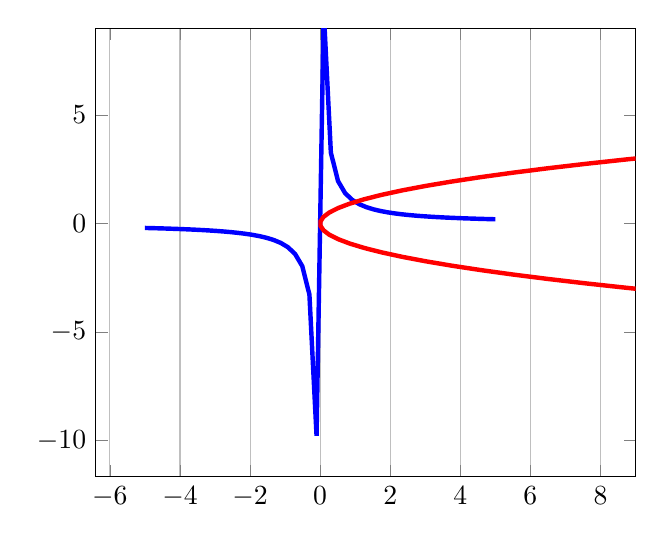
\begin{tikzpicture}
	\begin{axis}[xmajorgrids, xmax=9,ymax=9, samples=50]
	\addplot[blue, ultra thick] (x,1/x);
	\addplot[red,  ultra thick] (x*x,x);
	\end{axis}
	\end{tikzpicture}\\
	\vspace{2cm}
	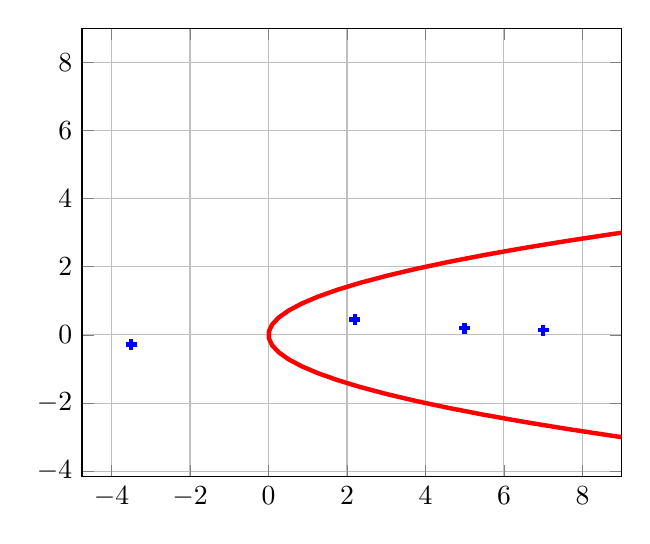
\begin{tikzpicture}
	\begin{axis}[grid, xmax=9,ymax=9, samples=50]
	\addplot[draw=none,mark=+,blue, ultra thick,samples at={-3.5,0,2.2,5,7}] (x,1/x);
	\addplot[red,  ultra thick] (x*x,x);
	\end{axis}
	\end{tikzpicture}\\
	
	\vspace{2cm}
	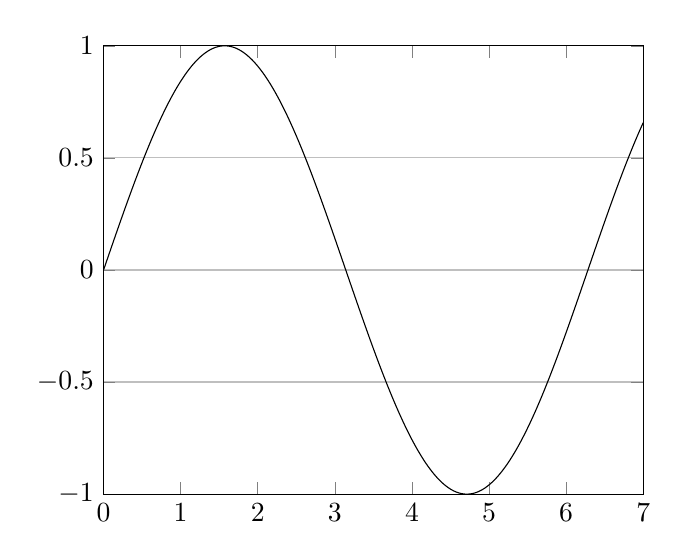
\begin{tikzpicture}
	\begin{axis}[ymajorgrids,xmin=0,xmax=7,ymin=-1,ymax=1, samples=500]
	\addplot[thin,domain=0:7]{sin(deg(x))};
	\end{axis}
	\end{tikzpicture}\\

	\begin{tikzpicture}
	\begin{axis}[ymajorgrids,xmin=0,xmax=7,ymin=-1,ymax=1, samples=500]
	\addplot[thin,domain=0:7]{sin(rad(x))};
	\end{axis}
	\end{tikzpicture}\\
		\vspace{2cm}
	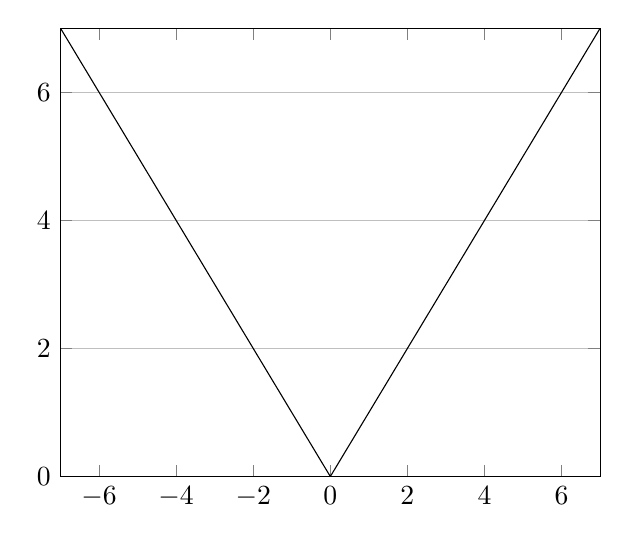
\begin{tikzpicture}
	\begin{axis}[ymajorgrids,xmin=-7,xmax=7,ymin=0,ymax=7, samples=500]
	\addplot[thin,domain=-7:7]{abs(x)};
	\end{axis}
	\end{tikzpicture}\\
		\vspace{2cm}
	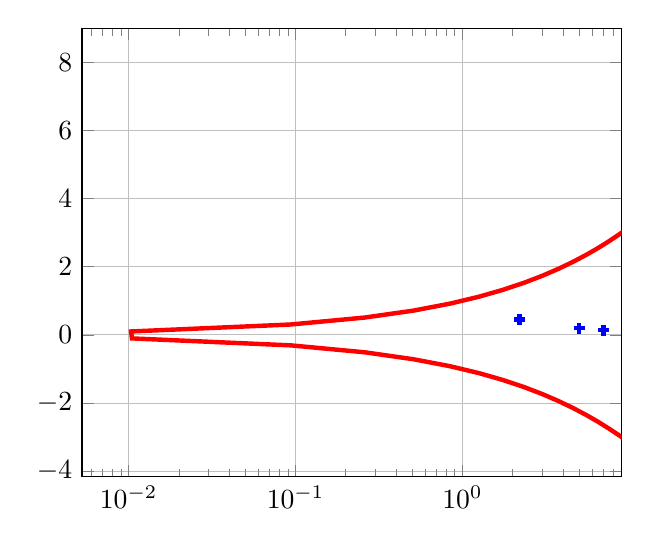
\begin{tikzpicture}
	\begin{semilogxaxis}[grid, xmax=9,ymax=9, samples=50]
	\addplot[draw=none,mark=+,blue, ultra thick,samples at={-3.5,0,2.2,5,7}] (x,1/x);
	\addplot[red,  ultra thick] (x*x,x);
	\end{semilogxaxis}
	\end{tikzpicture}\\
	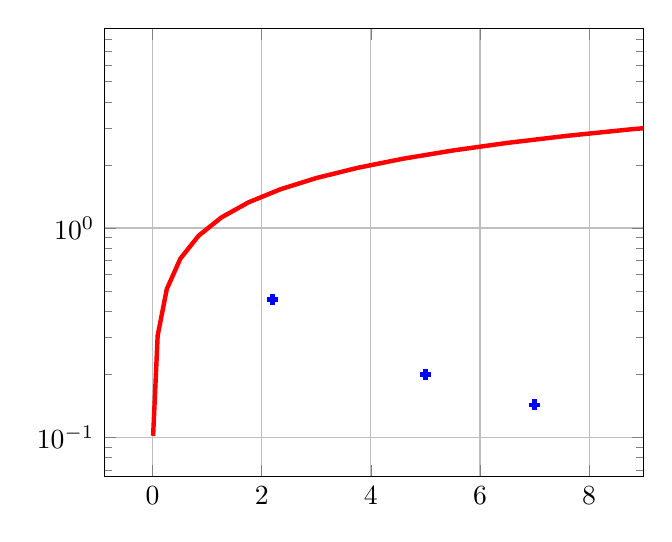
\begin{tikzpicture}
		\begin{semilogyaxis}[grid, xmax=9,ymax=9, samples=50]
		\addplot[draw=none,mark=+,blue, ultra thick,samples at={-3.5,0,2.2,5,7}] (x,1/x);
		\addplot[red,  ultra thick] (x*x,x);
		\end{semilogyaxis}
	\end{tikzpicture}\\
	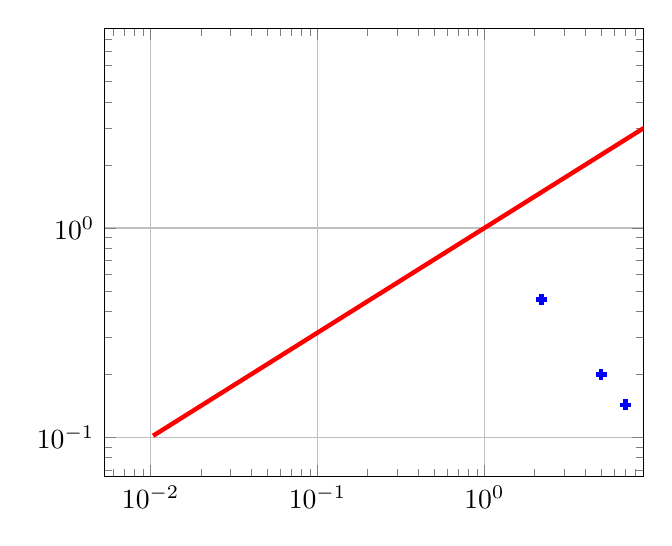
\begin{tikzpicture}
	\begin{loglogaxis}[grid, xmax=9,ymax=9, samples=50]
	\addplot[draw=none,mark=+,blue, ultra thick,samples at={-3.5,0,2.2,5,7}] (x,1/x);
	\addplot[red,  ultra thick] (x*x,x);
	\end{loglogaxis}
	\end{tikzpicture}\\
	\vspace{2cm}
	\begin{tikzpicture}
	\begin{axis}[ymajorgrids,xmin=0,xmax=7,ymin=-1,ymax=1, samples=500]
	%\addplot[thin,domain=0:7]{sin(\x x)};
	\end{axis}
	\end{tikzpicture}\\
	\usepgfplotslibrary{polar}
		\begin{tikzpicture}
		\begin{polaraxis}
		\addplot[domain=0:360,samples=300] {sin(6*x)}; 
		\end{polaraxis}
		\end{tikzpicture}
		
	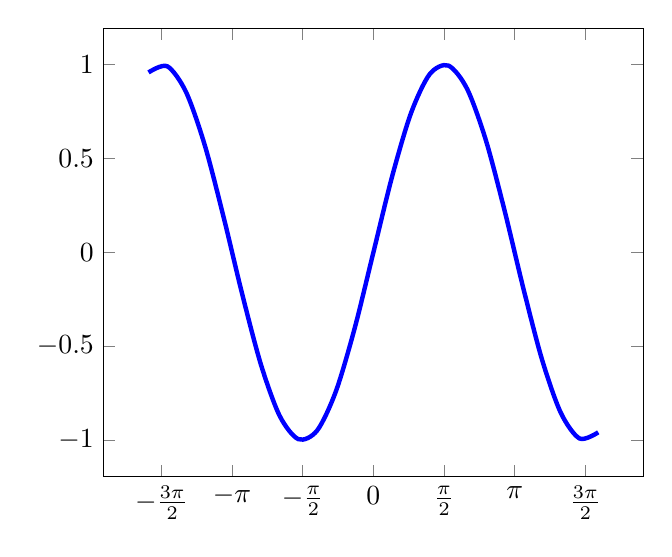
\begin{tikzpicture}
	\begin{axis}[xtick={
		-6.28318, -4.7123889, -3.14159, -1.5708,0,
		1.5708, 3.14159, 4.7123889, 6.28318
	},
	xticklabels={
		$-2\pi$, $-\frac{3\pi}{2}$, $-\pi$, $-\frac{\pi}{2}$,0,
		$\frac{\pi}{2}$, $\pi$, $\frac{3\pi}{2}$, $2\pi$
	}
	]
	\addplot [smooth,mark=none, ultra thick, blue] {sin(deg(x))};
	\end{axis}
	\end{tikzpicture}
\end{document}




